\documentclass[a4paper, 11pt]{article}
\usepackage[slovak]{babel}
\usepackage[utf8]{inputenc}
\usepackage[text={17cm, 24cm}, left=2cm, top=3cm]{geometry}
\usepackage[unicode]{hyperref}
\usepackage{graphics}
\usepackage{xcolor}
\usepackage{mathtools}

    
\begin{document}
    \begin{titlepage}
    	\begin{center}
    		\Huge
    			\textsc{Kalkulátor KAPUSTA} \\
                \vspace{\stretch{0.1}}
    		        Uživateľská príručka
    		    \vspace{\stretch{0.2}}
    		\begin{figure}[h]
    	        \centering
    		        \scalebox{0.6}{
\includegraphics{kapusta.png}}
    		\end{figure}
    		\vspace{\stretch{0.618}}
		\end{center}

		{\Large
			Kapustniaci \hfill 2021
		}
    \end{titlepage}
    
    \tableofcontents
    
    \newpage
    
    \section{Kalkulačka KAPUSTA}
        Kalkulačka s názvom KAPUSTA je program, určený na počítanie jednoduchých matematických\\ výpočtov. V tomto dokumente je základný popis funkcií kalkulačky, význami jednotlivých tlačidiel a spôsob inštalácie a odinštalácie programu. Pred prvým spustením je odporúčané si danú príručku preštudovať a vyhnúť sa tak problémom pri inštalácii, či používaní. Do zdrojového kódu nie je povolené zasahovať a meniť ho, pretože hrozí vznik problémov a následná nefunkčnosť programu.
    
    \newpage
    
    \section{Inštalácia kalkulačky}
        \subsection{Inštalácia na Windows}
            \subsubsection{Inštalácia pomocou inštalátoru}
            Po stiahnutí inštalátora ho spustíte. Ako prvé povolíte prípadné vykonávania zmien v zariadení. Následne si prečítate licenčné podmienky.
                \begin{figure}[h]
                    \centering
                        \scalebox{0.6}{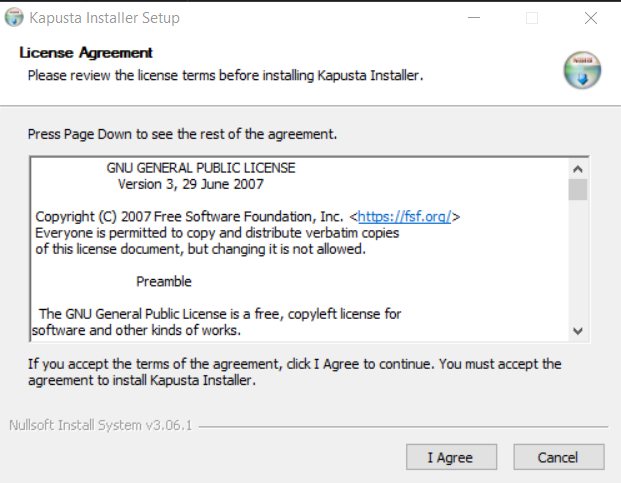
\includegraphics{licencia.png}}
                        \caption{License Agreement}
                \end{figure}
            \vspace{10mm}
            \\Vyberiete, kam chcete vytvoriť odkazy na aplikáciu.
                \begin{figure}[h]
                    \centering
                        \scalebox{0.6}{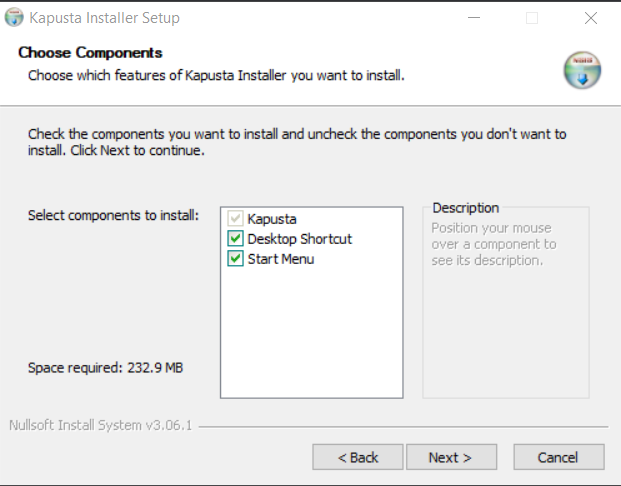
\includegraphics{components.png}}
                        \caption{Voľba záložiek}
                \end{figure}
            \\
            \\
            Potom zvolíte umiestnenie na disku, kam aplikáciu \verb|Kapusta| nainštalujete. Spustí sa inštalácia, po dokončení inštalácie zvoľte tlačidlo \verb|Close|. Ak všetko prebehlo správne, na zvolených miestach sa vám vytvoria sa ikony aplikácie. Po dvojkliknutí na ikonu sa program spustí a je pripravený na použitie.
            \begin{figure}[h]
                    \centering
                        \scalebox{1}{
\includegraphics{ikona.png}}
                        \caption{Ikona vytvorená na ploche}
                \end{figure}
            \subsubsection{Manuálna inštalácia}
            Stiahnete \verb|.zip| súbor. Rozbalíte ho a spustíte program \verb|kapusta.exe|.
            \newpage
        \subsection{Inštalácia na Linux}
            \subsubsection{Inštalácia pomocou inštalátoru}
                Spustíte stiahnutý súbor na inštaláciu a nainštalujete.  
                \begin{figure}[h]
                    \centering
                        \scalebox{0.6}{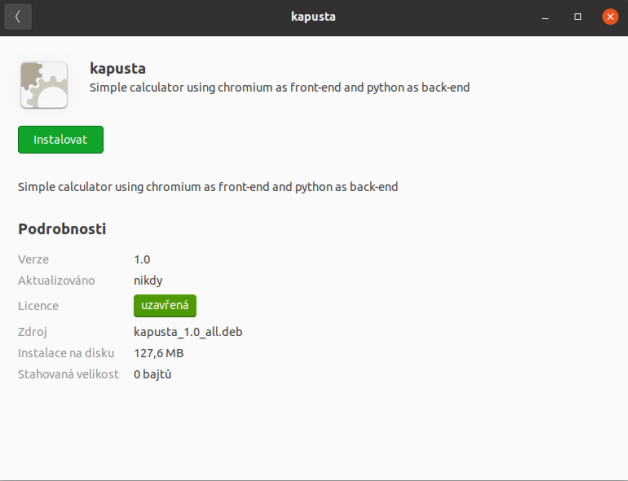
\includegraphics{linux5.png}}
                        \caption{Inštalácia na Linux}
                \end{figure}
                \vspace{10mm}
                \\Pres spustením inštalácie bude od vás vyžadované heslo, zadáte ho a inštalácia sa spustí.
                    \begin{figure}[h]
                        \centering
                            \scalebox{0.6}{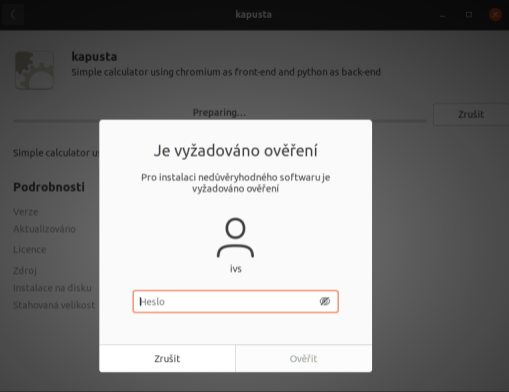
\includegraphics{linux4.png}}
                            \caption{Požadovanie hesla}
                    \end{figure}
                \\
                Po nainštalovaní je aplikácia pripravená na použitie.
                \newpage    
            \subsubsection{Manuálna inštalácia}
                Stiahnutý súbor umiestníte do ľubovoľného, ale vhodného priečinka. Následné cez terminál napíšete príkaz:\\
                \verb|sudo apt install ./kapusta_1.0_all.deb| \\
                a spustí sa inštalácia. 
                \begin{figure}[h]
                    \centering
                        \scalebox{0.7}{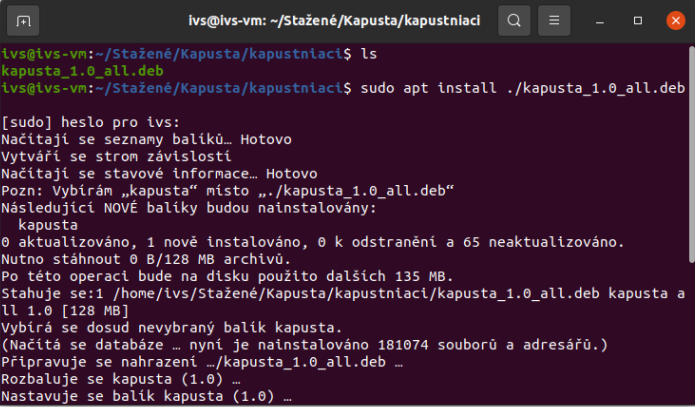
\includegraphics{linux1.png}}
                        \caption{Priebeh inštalácie}
                \end{figure}
                \\Aplikácia sa  spustí príkazom\\
                \textbf{kapusta} \\
                a je pripravená na použitie.
                \begin{figure}[h]
                    \centering
                        \scalebox{0.6}{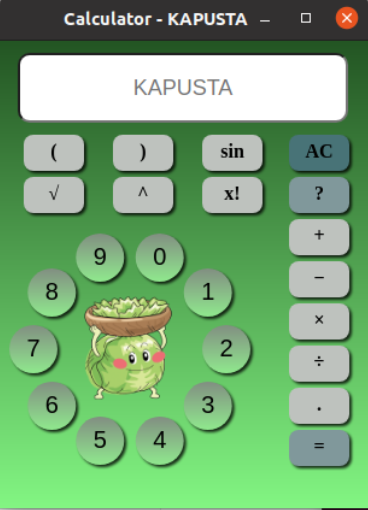
\includegraphics{linux2.png}}
                        \caption{Aplikácia v Linux prostredí}
                \end{figure}
                    
                    
        
    \newpage
        
    \section{Vzhľad kalkulačky a rozloženie jej prvkov}
        \begin{enumerate}
            \color{blue}
            \item displej,
            \color{red}
            \item tlačidlá s číslami 0 - 9,
            \color{green}
            \item nápoveda,
            \color{yellow}
            \item tlačidlá s funkciami
            \color{purple}
            \item AC tlačidlo
        \end{enumerate}
        \vspace{15mm}
        \begin{figure}[h]
    		        \centering
    			        \scalebox{0.7}{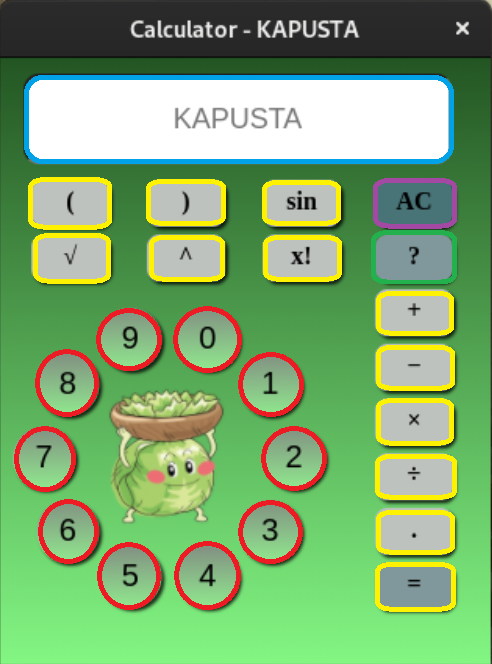
\includegraphics{popis.png}}
    			        \caption{Kalkulačka s vyznačenými tlačidlami podľa farieb}
    	\end{figure}
    	
    \newpage
    
    \section{Funkcie a práca s kalkulačkou}
        Kalkulačku je možné ovládať pomocou myši kliknutím na jednotlivé tlačidlá alebo stlačením príslušnej klávesy na klávesnici.
        
        \subsection{Tlačidlá 0 - 9 (Na klávesnici klávesy 0 - 9)}
        \begin{itemize}
            \item po kliknutí na tlačidlo s číslom sa dané číslo zobrazí na displeji.
        \end{itemize}
        
        \subsection{Tlačidlo + (na klávesnici klávesa “+”)}
        \begin{itemize}
            \item Reprezentuje funkciu sčítanie a vyžaduje dve alebo viac čísel na sčítanie, kde číslo môže byť celé alebo desatinné(tlačidlo .), kladné alebo záporné,
            \item príklad vstupov:  “3 + 4” , “3 + 4 + 6”
            
        \end{itemize}
        
         \subsection{Tlačidlo - (na klávesnici klávesa -)}
        \begin{itemize}
            \item Reprezentuje funkciu odčítanie a vyžaduje dve alebo viac čísel na sčítanie, kde číslo môže byť celé alebo desatinné(viď tlačidlo .), kladné alebo záporné,
            \item príklad vstupov:  “3 - 4” , “3 - 4 - 6”
        \end{itemize}
        
         \subsection{Tlačidlo x (na klávesnici klávesa *)}
        \begin{itemize}
            \item Reprezentuje funkciu násobenie a vyžaduje dve alebo viac čísel na násobenie, kde číslo môže byť celé alebo desatinné(viď tlačidlo .), kladné alebo záporné,
            \item príklad vstupov:  “3 - 4” , “3 - 4 - 6”
        \end{itemize}
        
         \subsection{Tlačidlo / (na klávesnici klávesa /)}
        \begin{itemize}
            \item Reprezentuje funkciu delenie a vyžaduje dve alebo viac čísel na násobenie, kde číslo môže byť celé alebo desatinné(viď tlačidlo .), kladné alebo záporné,
            \item príklad vstupov:  “3 / 4” , “3 / 4 / 6”
        \end{itemize}
        
        \subsection{Tlačidlo \^\ (na klávesnici klávesa \^\ )}
        \begin{itemize}
            \item Reprezentuje funkciu “mocnina s prirodzeným exponentom”, kde exponent je prirodzené číslo a základ reálne číslo,
            \item Príklad vstupov:  “3 \^\ 4” , “3.5 \^\ 4”
        \end{itemize}
        
        \subsection{Tlačidlo n$\surd$x (na klávesnici $\surd$)}
        \begin{itemize}
            \item Reprezentuje funkciu “všeobecná odmocnina”, kde n, x sú nezáporné reálne čísla,
            \item príklad vstupov:  “3$\surd$27”
        \end{itemize}
        
        \subsection{Tlačidlo x! (na klávesnici klávesa !)}
        \begin{itemize}
            \item Reprezentuje funkciu “faktoriál”, kde x je celé nezáporné číslo,
            \item príklad vstupov:  “3!”
        \end{itemize}
        
        \subsection{Tlačidlo sin (na klávesnici “sin”)}
        \begin{itemize}
            \item Reprezentuje funkciu “sinus”, kde x je reálne číslo,
            \item príklad vstupov:  “sin(0.5)”
        \end{itemize}
        
        \subsection{Tlačidlá ( ) (na klávesnici “( )”)}
        \begin{itemize}
            \item reprezentujú prioritu operácii, zápis je platný ak je ľavá zátvorka vždy ukončená pravou,
            \item príklad vstupov: “3 * (5 - 2)”  $\rightarrow$ najskôr sa vyhodnotí odčítanie a
            následne sa výsledok odčítania vynásobi troma
        \end{itemize}
        
    	\subsection{Tlačidlo . (na klávesnici “.”)}
        \begin{itemize}
            \item Reprezentuje desatinnú čiarku, pre možnosť počítať aj s desatinnými číslami,
            \item ! používať bodku, nie čiarku na klávesnici !
            \item príklad vstupov:  “0.5”, “6.9”
        \end{itemize}
        
        \subsection{Tlačidlo = (na klávesnici klávesa “enter”)}
        \begin{itemize}
            \item Reprezentuje ukončenie výrazu a následne sa zobrazí na displeji výsledok daného výrazu,
            \item je nutné dané tlačidlo použit pri konci každého výpočtu
        \end{itemize}
        
        \subsection{Tlačidlo AC (na klávesnici klávesa “Delete”)}
        \begin{itemize}
            \item Vymaže obsah zobrazený na displeji,
            \item všetky predchádzajúce výpočty sa vymažú.
        \end{itemize}
        
        \subsection{Klávesa “Backspace”}
        \begin{itemize}
            \item Vymaže posledný vložený znak na displeji,
            \item táto možnosť je dostupná len pri ovládaní pomocou klávesnice.
        \end{itemize}
        
        \subsection{Tlačidlo ? (na klávesnici klávesa “F2”)}
        \begin{itemize}
            \item Reprezentuje zobrazenie nápovedy, ktorá sa uživateľovi objaví po stlačení tohto tlačidla.
        \end{itemize}

        \newpage
        
         
        \section{Odinštalácia kalkulačky}
            \subsection{Odinštalácia na Windows}
                V ponuke štart nájdete aplikáciu \verb|Kapusta|, kliknete pravým tlačidlom a zvolíte možnosť odinštalovať.
                \begin{figure}[h]
                        \centering
                            \scalebox{1}{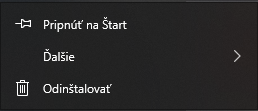
\includegraphics{uninstall.png}}
                            \caption{Odinštalácia na Windows}
                    \end{figure}
                \\
                Otvorí sa okno so všetkými nainštalovanými programami v počítači, nájdete názov \verb|Kapusta|\\ a odinštalujete.
            \subsection{Odinštalácia na Linux}
                Program v OS Linux odinštalujeme 2 spôsobmi. Cez príkazový riadok s príkazom:\\
                \textbf{sudo apt remove kapusta}\\
                alebo vyhľadáme aplikáciu v počítači a po otvorení klikneme na možnosť \verb|Odebrat|.
                \begin{figure}[h]
                    \centering
                        \scalebox{0.6}{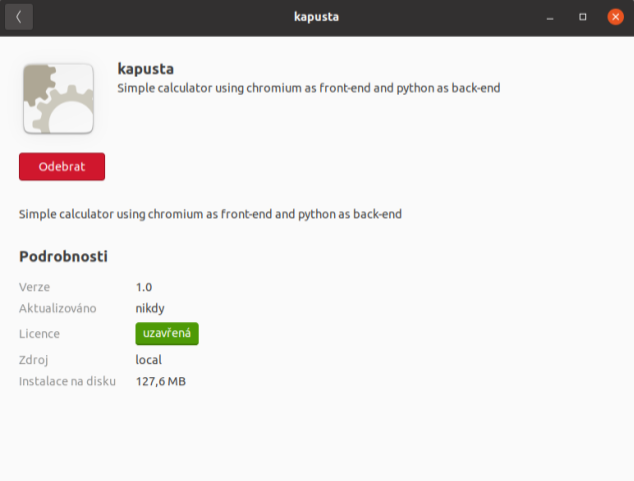
\includegraphics{linux3.png}}
                        \caption{Odinštalácia na Linux}
                \end{figure}
                \\Po kliknutí odinštaluje program Kapusta z počítaču.
 
    \newpage 
        
        \thispagestyle{empty}
        \begin{figure}[t]
    	    \centering
                \scalebox{0.5}{
\includegraphics{logo.png}}
    	        \caption{Logo kalkulačky}
    	\end{figure}
    	\begin{figure}[h]
            \centering
    	        \scalebox{0.5}{
\includegraphics{qr.png}}
    	        \caption{QR kód ku zdrojovému kódu}
    	        \vspace{30mm}
    	        {\small
			    Tím Kapustniaci - FIT VUT Brno \hfill 2021
		        }
    	\end{figure}
\end{document}
